\chapter{Analisi dei risultati}

\section{Training e validation}
Con l'architettura presentata e una volta pronto il codice necessario, è stato possibile procedere con il training della rete e con la successiva valutazione dei risultati.
Gli iperparametri dell'addestramento sono stati impostati nel seguente modo:
\begin{itemize}
    \item durata del training: 50 epoche
    \item learning rate: 0.001
    \item batch size: 32, il più alto possibile con la memoria GPU a disposizione.
    \item loss function: MSE
\end{itemize}
In figura \ref{training} e \ref{validation} sono mostrati i grafici degli andamenti del loss di training e validation.
\begin{figure}[H]
    \centering
    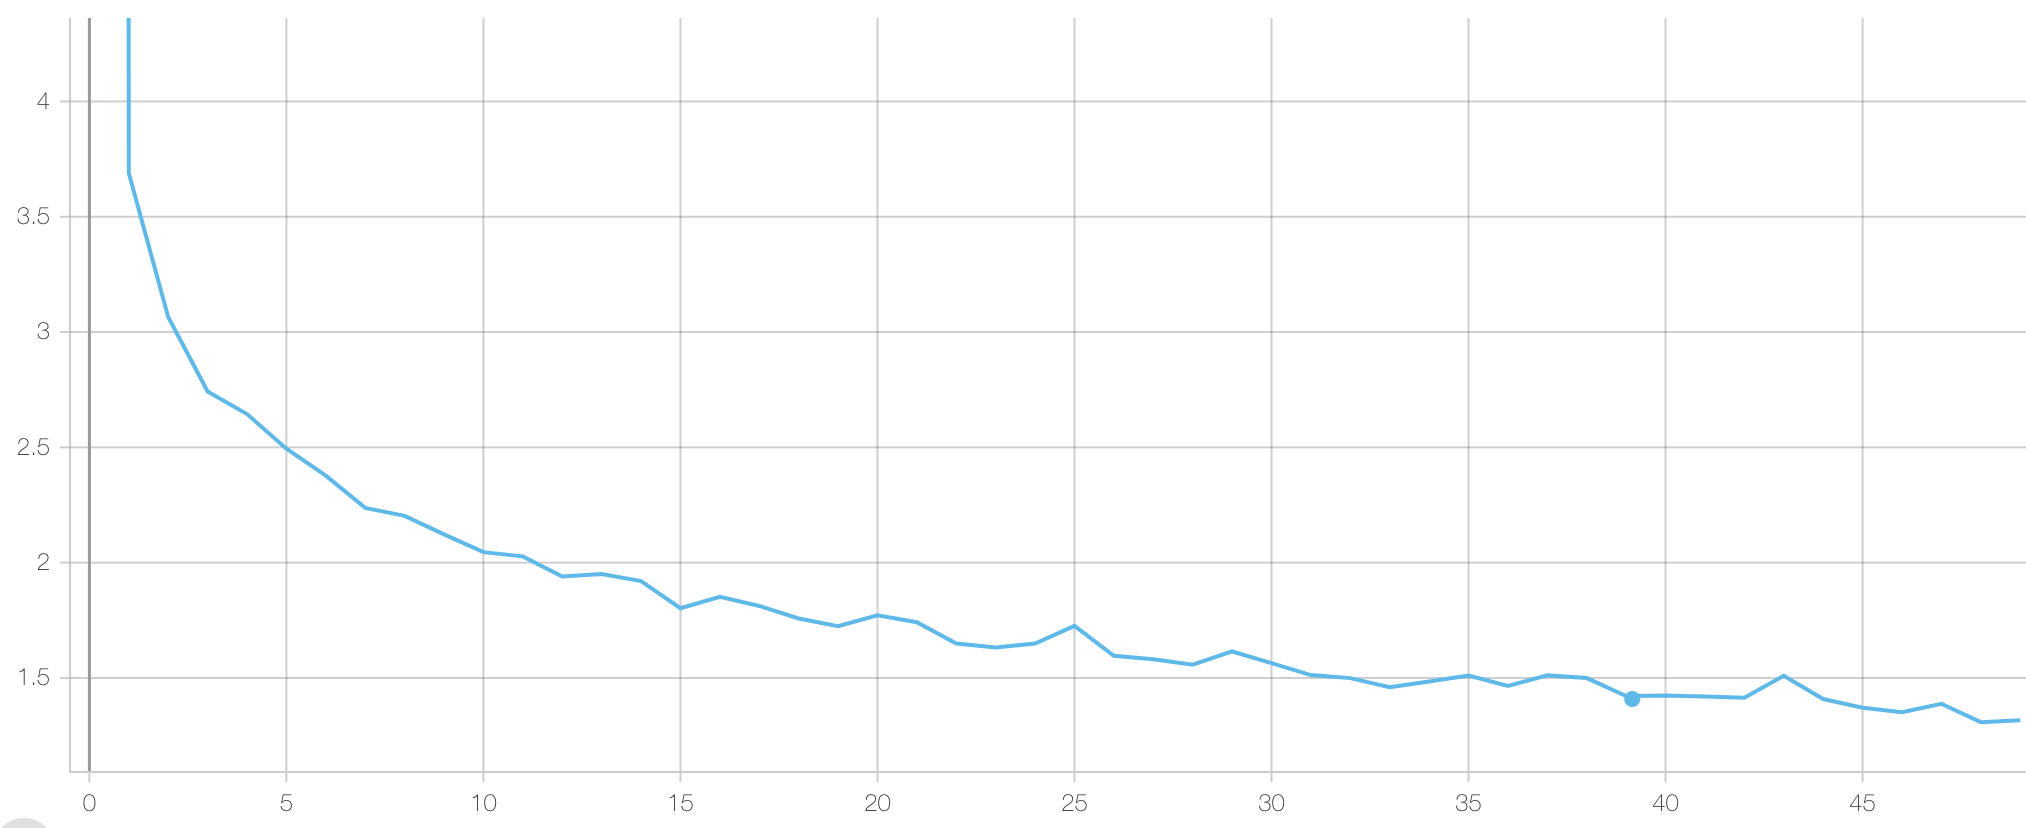
\includegraphics[width=1.0\columnwidth]{final_training.png}
    \caption[Andamento del training loss]{Andamento del training loss}
    \label{training}
\end{figure}

\begin{figure}[H]
    \centering
    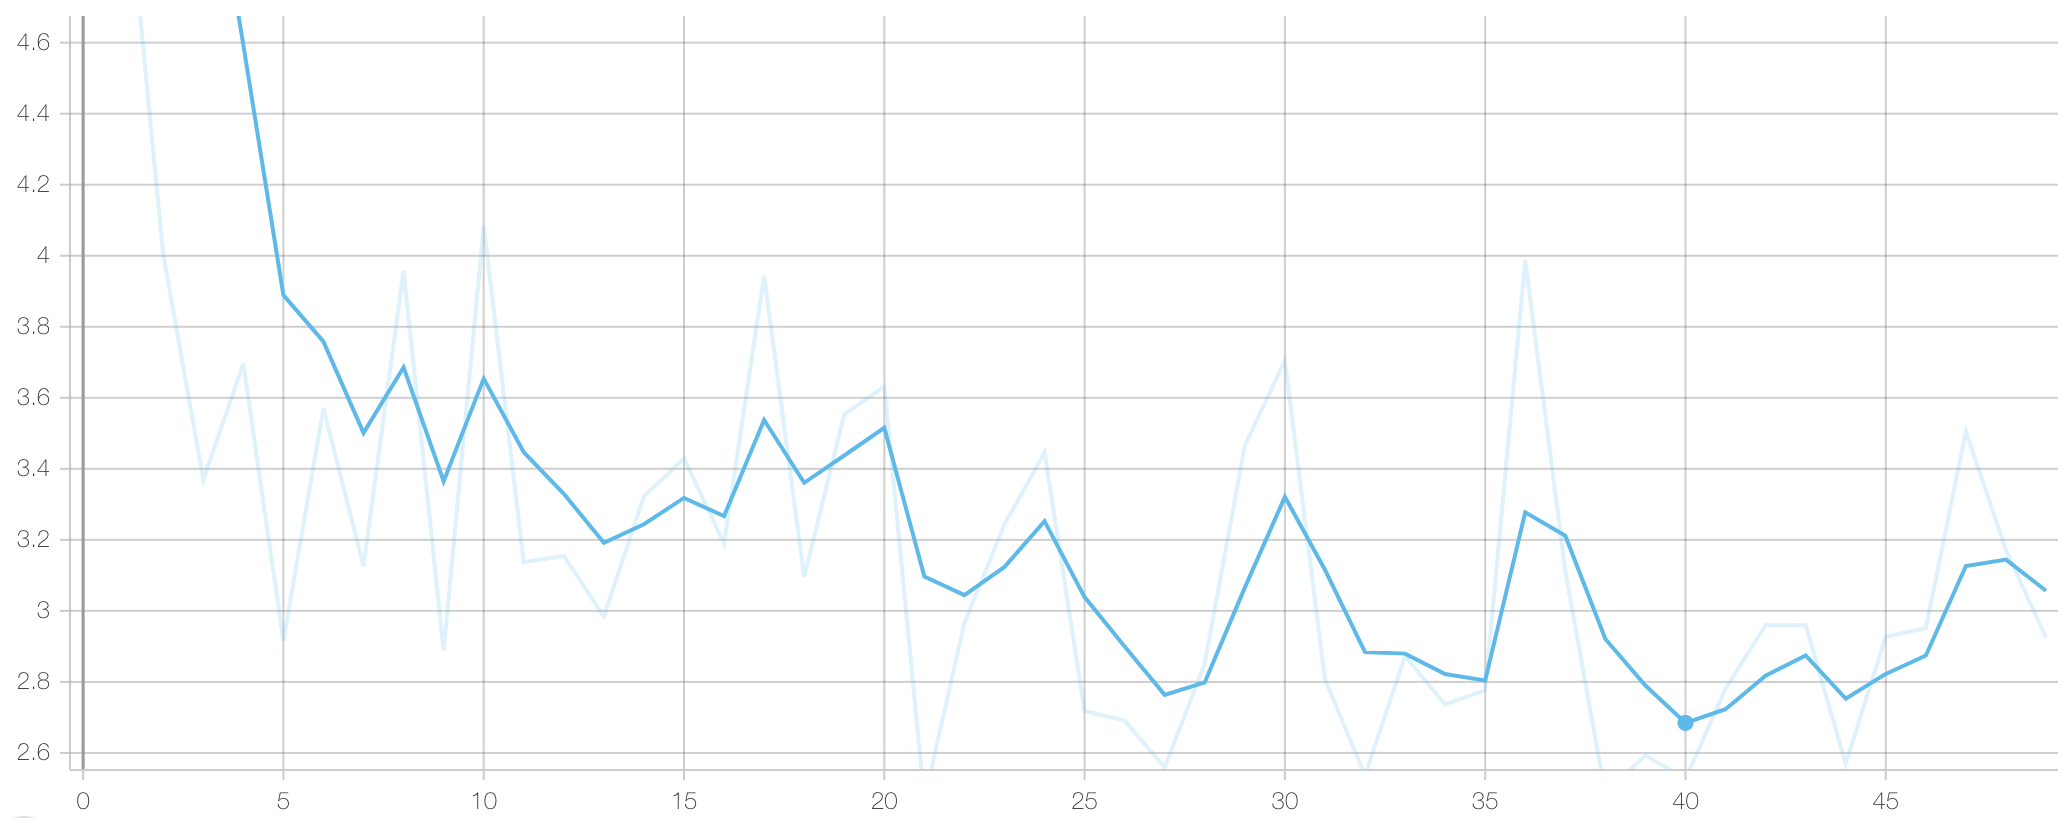
\includegraphics[width=1.0\columnwidth]{final_validation.png}
    \caption[Andamento del validation loss]{Andamento del validation loss}
    \label{validation}
\end{figure}

\section{Test e risultati sperimentali}
Nelle figure seguenti sono mostrati alcuni risultati sperimentali della rete addestrata. La prima e la seconda colonna mostrano gli input ToF e Stereo rispettivamente. Si nota nei dati ToF la presenza di alcuni "buchi" sulle superfici poco riflettenti e sulle regioni affette dal "multipath error", ossia in prossimità delle zone di incidenza tra le superfici. Per quanto riguarda lo stereo, si notano in particolare accuratezze limitate sui bordi.\\
La terza colonna mostra la fusione, ossia l'output della rete. Infine nella quarta colonna vengono illustrati i ground truth. La fusione è in grado di estrarre le informazioni più accurate da entrambe le sorgenti, tappando le lacune del ToF ed eliminando gli artefatti lungo i bordi dello stereo. \\

\noindent\makebox[\linewidth][s]{\textbf{ | ToF Input | Stereo Input | Output Disparity | Ground Truth |}}\\
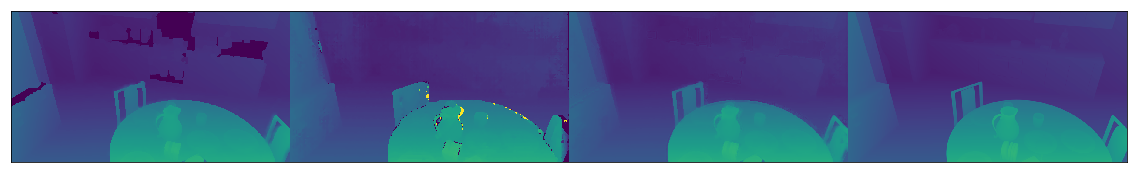
\includegraphics[width=1.0\columnwidth]{test_fig_1.png}
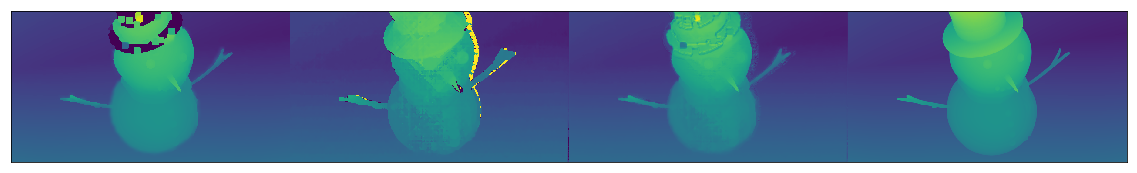
\includegraphics[width=1.0\columnwidth]{test_fig_2.png}

\includegraphics[width=1.0\columnwidth]{test_fig_3.png}
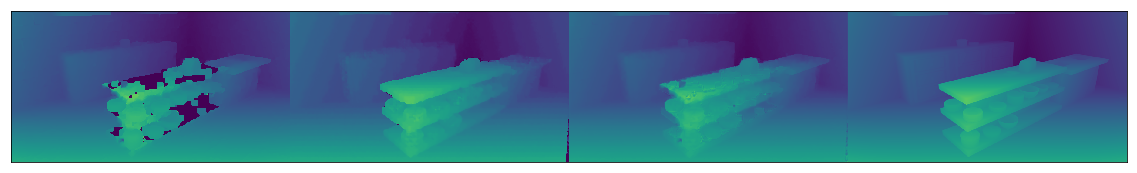
\includegraphics[width=1.0\columnwidth]{test_fig_4.png}

\section{Confronti tra differenti architetture}
\paragraph{La nostra rete contro una rete elementare}Confrontiamo ora i risultati che abbiamo ottenuto contro quelli acquisiti da una semplice rete illustrata in figura \ref{simple_net}. Questa architettura non include blocchi residuali, normalizzazioni e convoluzioni dilatate.
\begin{figure}[ht]
    \centering
    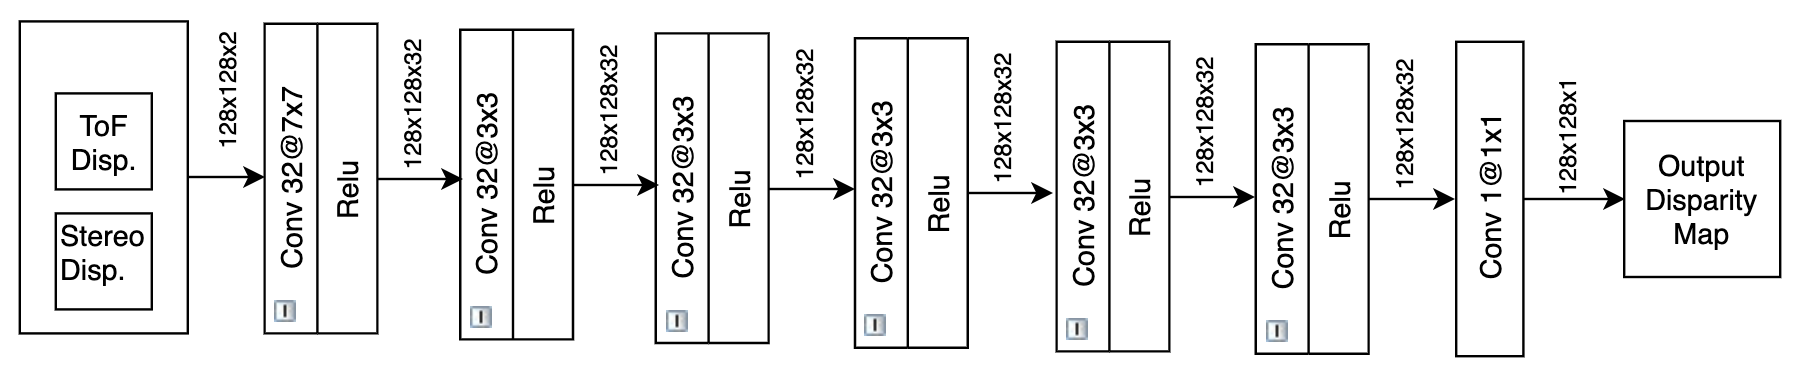
\includegraphics[width=1.0\columnwidth]{simple_net.png}
    \caption{Diagramma di una semplice CNN senza blocchi residuali, convoluzioni dilatate e normalizzazioni}
    \label{simple_net}
\end{figure}

\begin{figure}[ht]
    \centering
    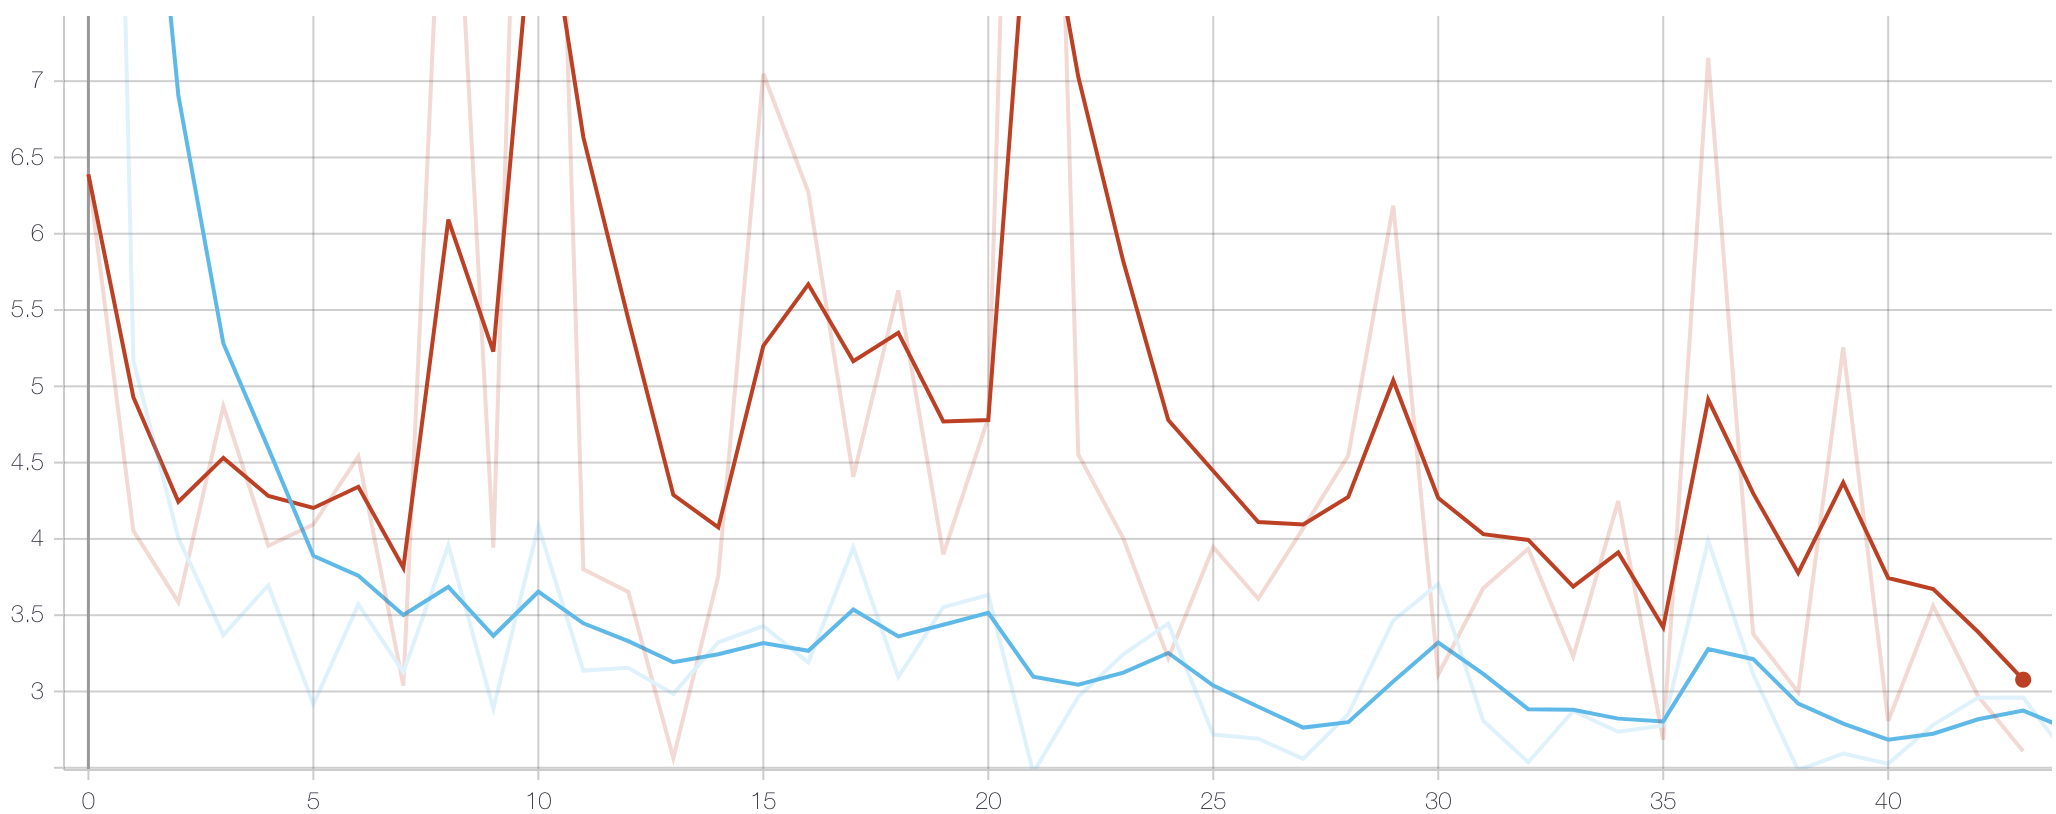
\includegraphics[width=0.8\columnwidth]{simplenet_vs_final.png}
    \caption[Confronto del validation loss della nostra architettura contro una versione più elementare]{
        Confronto del validation loss della nostra architettura contro una versione più elementare. \\
        \fcolorbox{black}{cyan}{\rule{0pt}{6pt}\rule{6pt}{0pt}}\quad DRFNet (figura \ref{my_net})\\
        \fcolorbox{black}{red}{\rule{0pt}{6pt}\rule{6pt}{0pt}}\quad La CNN elementare (figura \ref{simple_net})
    }
    \label{simplevsfinal}
\end{figure}

Si nota immediatamente dalla figura \ref{simplevsfinal} che la nostra rete performa assai meglio della rete con architettura elementare convergendo molto più rapidamente e con meno oscillazioni.

\paragraph{Convoluzione dilatata contro senza dilatazione} Proviamo ora a togliere la dilatazione dagli strati di convoluzione della nostra rete. Proviamo quindi a comparare i risultati così ottenuti con i risultati ottenuti con la dilatazione.
\begin{figure}[H]
    \centering
    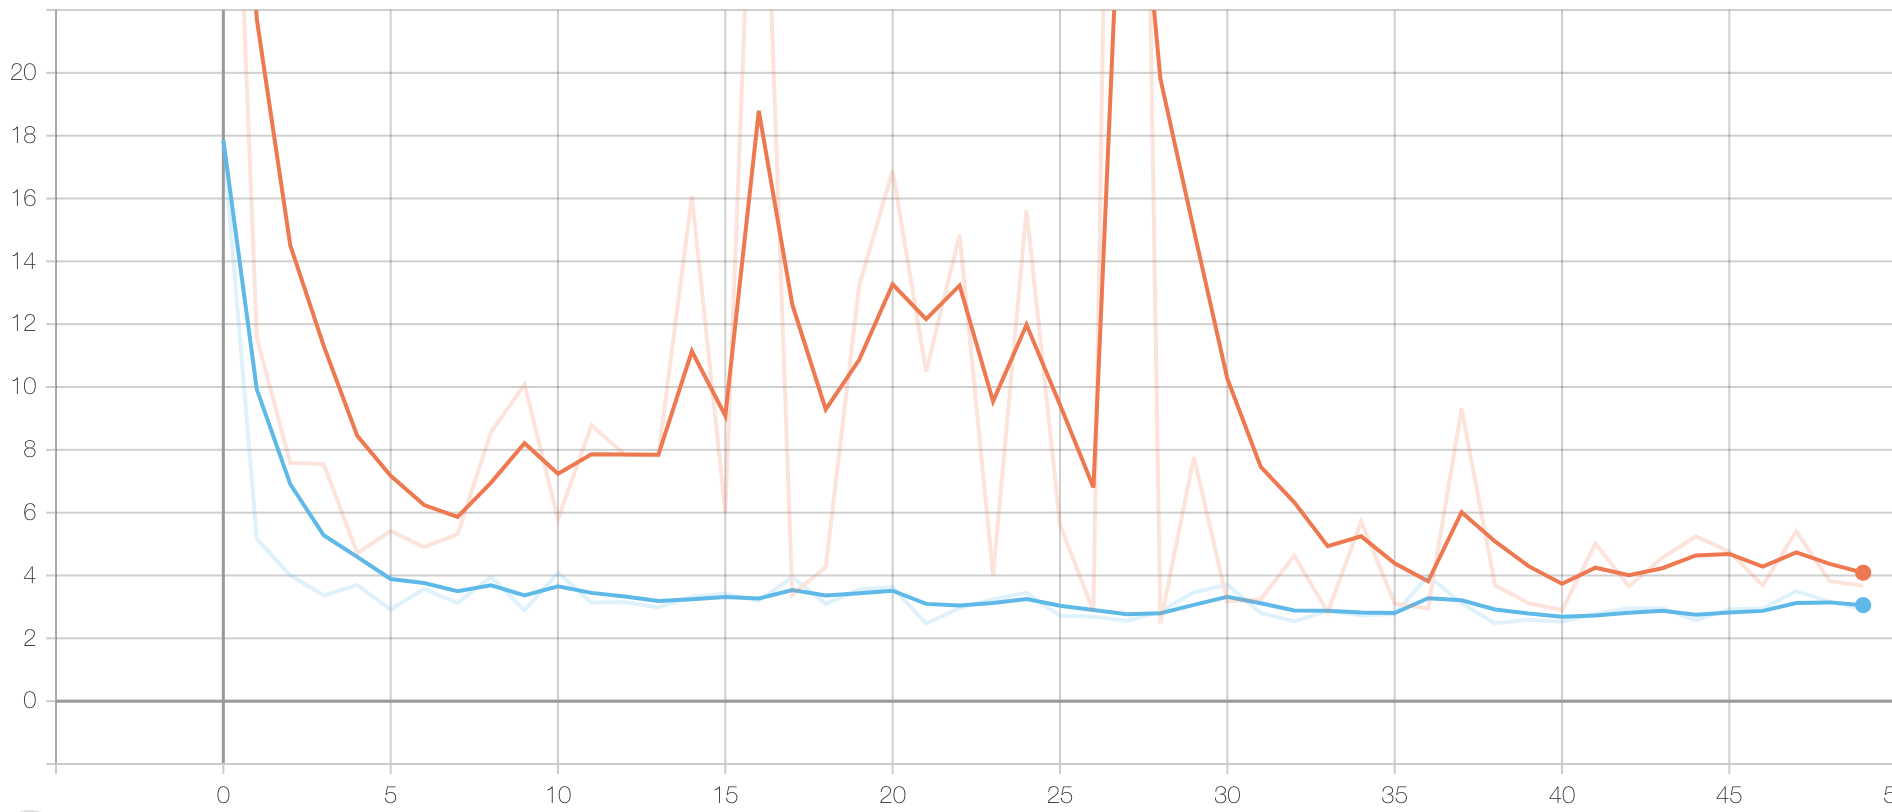
\includegraphics[width=0.8\columnwidth]{dilation_vs_nodilation.png}
    \caption[Confronto del validation loss della rete con strati di convoluzione dilatata contro senza dilatazione]{
        Confronto del validation loss della rete con strati di convoluzione dilatata contro senza dilatazione. \\
        \fcolorbox{black}{cyan}{\rule{0pt}{6pt}\rule{6pt}{0pt}}\quad DRFNet (figura \ref{my_net})\\
        \fcolorbox{black}{orange}{\rule{0pt}{6pt}\rule{6pt}{0pt}}\quad La rete senza dilatazione sulla convoluzione
    }
    \label{dilation_vs_nodilation}
\end{figure}
Come si vede dalla figura \ref{dilation_vs_nodilation}, la dilatazione negli strati di convoluzione ha un effetto positivo sulle performance della rete sul validation set. È possibile difatti apprezzare un andamento migliore nel caso dell'utilizzo della dilatazione.

\paragraph{Comparazioni tra diverse profondità della rete}
Con l'obiettivo di determinare la migliore profondità della rete, proviamo a variare il numero di blocchi residuali tra 4, 6 e 8. 
\begin{figure}[H]
    \centering
    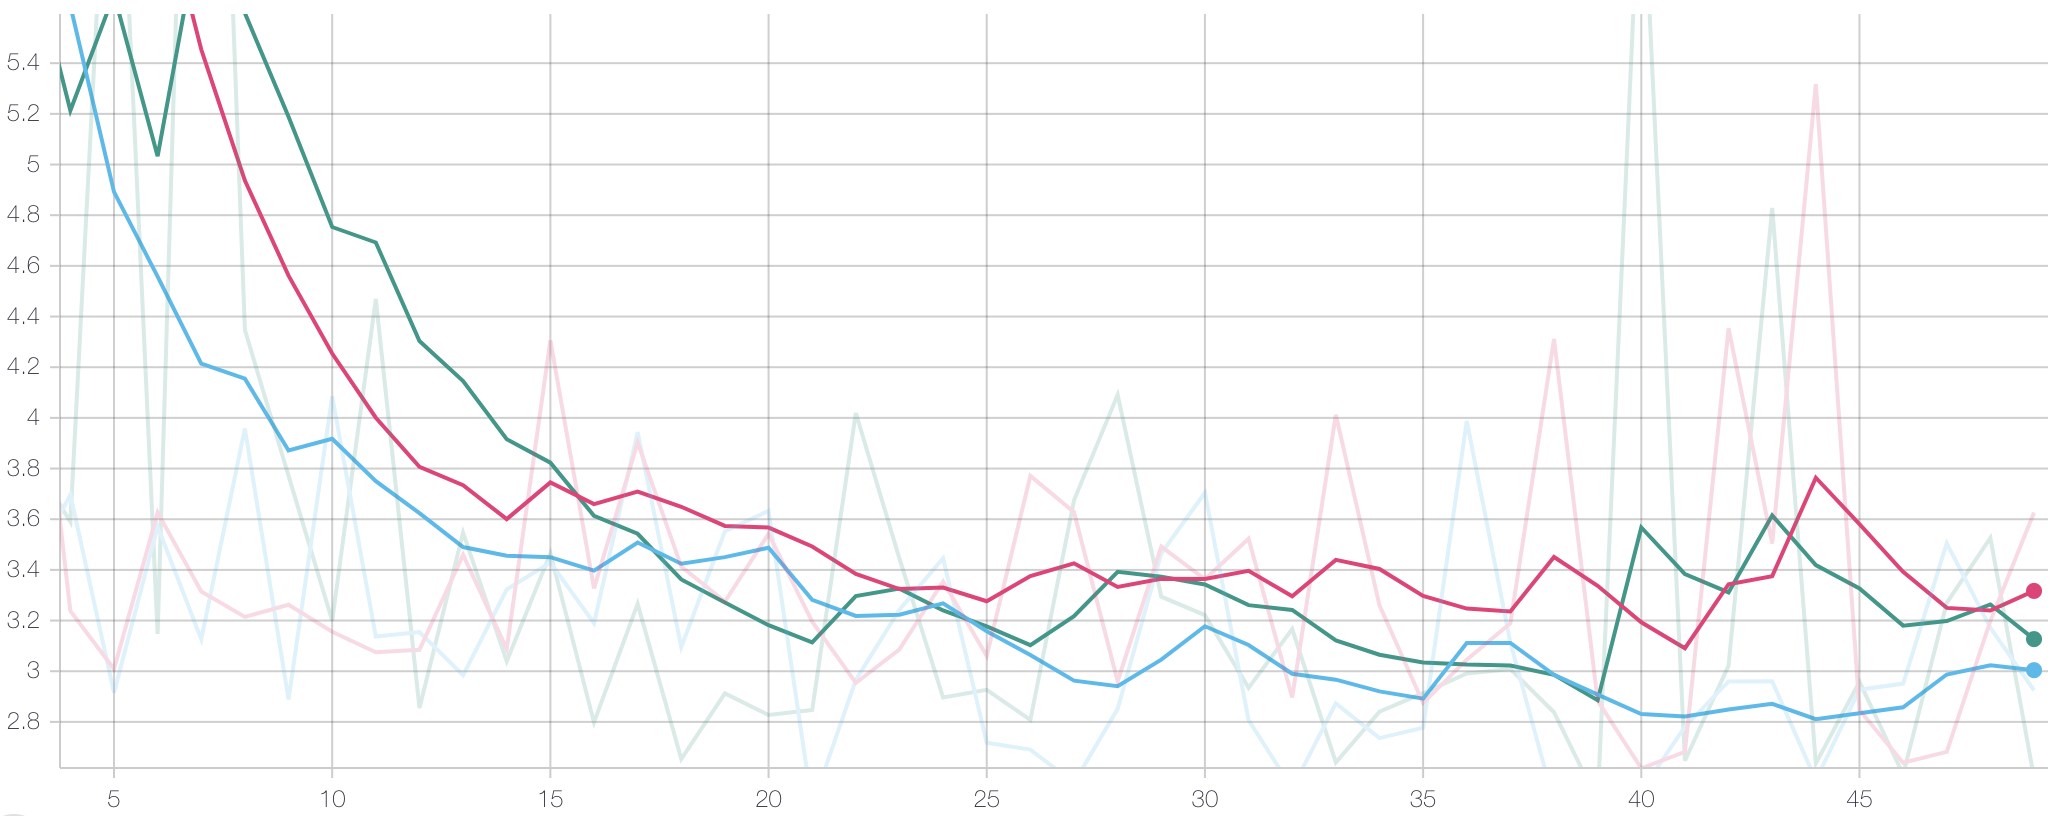
\includegraphics[width=0.8\columnwidth]{depth_compare.png}
    \caption[Confronto tra differenti numeri di blocchi residuali]{
        Confronto tra differenti numeri di blocchi residuali. \\
        \fcolorbox{black}{cyan}{\rule{0pt}{6pt}\rule{6pt}{0pt}}\quad 6 blocchi residuali\\
        \definecolor{mycolor1}{RGB}{219,70,119}
        \definecolor{mycolor2}{RGB}{67,150,176}
        \fcolorbox{black}{mycolor1}{\rule{0pt}{6pt}\rule{6pt}{0pt}}\quad 4 blocchi residuali\\
        \fcolorbox{black}{mycolor2}{\rule{0pt}{6pt}\rule{6pt}{0pt}}\quad 8 blocchi residuali
    }
    \label{depth_compare}
\end{figure}
Dal grafico comparativo di figura \ref{depth_compare} si vede un andamento leggermente migliore nel caso dell'utilizzo di 6 blocchi residuali, con 8 blocchi si hanno risultati molto simili mentre il caso peggiore è quello con 4 blocchi.